%===============================================================================
\chapter{Virtual Reference Feedback Tunning}
\label{chapter:vfrt}
%===============================================================================
\TODO:: REVER ESTE PARAGRAFO:

Em aplica��es pr�ticas, a descri��o matem�tica da planta n�o � dispon�vel e o sistema deve ser identificado
baseado nas medidas obtidas deste sistema. Este assunto tem atra�do a aten��o de diversos engenheiros de
controle desde 1940 com o pioneiro trabalho de Ziegler e Nichols (1942) com ajuste de controladores PID
industriais. Depois do trabalho de Ziegler e Nichols diversos trabalhos surgiram, muitos em formas de
aperfei�oamento e extens�es das t�cnicas j� apresentadas, e algumas com desenvolvimentos em novas dire��es
(\cite{mcmillan1983tuning}, \cite{Haalman1965}). A caracter�stica principal destes m�todos � que eles podem
ser facilmente utilizados: simples experimentos sobre a planta s�o executados e simples regras 
s�o aplicadas sobre os dados obtidos. O m�todo VRFT que ser� abordado aqui tem algumas destas 
caracter�sticas, pois s� requer que apenas um experimento seja executado sobre a planta. 
\cite{campi_leccini_savaresi2002}

%===============================================================================
%===============================================================================
\section{Controle baseado em dados}
\label{sec:vrft_control_data_based}
%===============================================================================

O projeto de controladores baseados em dados consiste obter ou ajustar os parametros de um modelo
para os controladores, baseado nos dados obtidos da planta em an�lise. Os dados utilizados para esta
tarefa s�o basicamente o sinal de entrada e sa�da do sistema.

Como j� foi discutido na se��o (\ref{sec:si_project_experiments}) estes dados podem ser obtidos de
diversas formas. Algumas vezes estas informa��es podem ser a opera��o normal da planta em malha
fechada com a presen�a de algum controlador, situa��o esta que tem um apelo grande em plantas
industriais, onde a parada do processo para levantamento de informa��es � indesejavel, e muitas
vezes at� invi�vel. Se existe a poss�bilidade de parar a planta e aplicar-se sinais predeterminados,
o projeto de experimentos pode trazer muitas vantagens.

\begin{figure}[htbp]
\center
\scalebox{1} % Change this value to rescale the drawing.
{
\begin{pspicture}(0,-1.1092187)(9.868125,1.1292187)
\pscircle[linewidth=0.04,dimen=outer](1.4,-0.08921875){0.2}
\psframe[linewidth=0.04,dimen=outer](4.4,0.31078124)(2.6,-0.48921874)
\psframe[linewidth=0.04,dimen=outer](7.2,0.31078124)(5.6,-0.48921874)
\pscircle[linewidth=0.04,dimen=outer](8.4,-0.08921875){0.2}
\psline[linewidth=0.04cm,arrowsize=0.05291667cm 2.0,arrowlength=1.4,arrowinset=0.4]{->}(0.0,-0.08921875)(1.2,-0.08921875)
\psline[linewidth=0.04cm,arrowsize=0.05291667cm 2.0,arrowlength=1.4,arrowinset=0.4]{->}(1.6,-0.08921875)(2.6,-0.08921875)
\psline[linewidth=0.04cm,arrowsize=0.05291667cm 2.0,arrowlength=1.4,arrowinset=0.4]{->}(4.4,-0.08921875)(5.6,-0.08921875)
\psline[linewidth=0.04cm,arrowsize=0.05291667cm 2.0,arrowlength=1.4,arrowinset=0.4]{->}(7.2,-0.08921875)(8.2,-0.08921875)
\psline[linewidth=0.04cm,arrowsize=0.05291667cm 2.0,arrowlength=1.4,arrowinset=0.4]{->}(8.4,0.7107813)(8.4,0.11078125)
\psline[linewidth=0.04cm,arrowsize=0.05291667cm 2.0,arrowlength=1.4,arrowinset=0.4]{->}(8.6,-0.08921875)(9.8,-0.08921875)
\psline[linewidth=0.04cm,arrowsize=0.05291667cm 2.0,arrowlength=1.4,arrowinset=0.4]{<-}(1.4,-0.28921875)(1.4,-1.0892187)
\psline[linewidth=0.04cm](1.4,-1.0892187)(9.2,-1.0892187)
\psline[linewidth=0.04cm](9.2,-1.0892187)(9.2,-0.08921875)
\usefont{T1}{ptm}{m}{n}
\rput(1.1126562,0.22078125){+}
\usefont{T1}{ptm}{m}{n}
\rput(8.112657,0.22078125){+}
\usefont{T1}{ptm}{m}{n}
\rput(8.112657,-0.37921876){+}
\usefont{T1}{ptm}{m}{n}
\rput(1.6473438,-0.37921876){-}
\usefont{T1}{ptm}{m}{n}
\rput(0.47,0.21078125){\small $r(t)$}
\usefont{T1}{ptm}{m}{n}
\rput(3.59,-0.08921875){\small $C(z, \rho)$}
\usefont{T1}{ptm}{m}{n}
\rput(6.36,-0.10921875){\small $G_0(z)$}
\usefont{T1}{ptm}{m}{n}
\rput(5.11,0.21078125){\small $u(t)$}
\usefont{T1}{ptm}{m}{n}
\rput(2.21,0.21078125){\small $\xi(t)$}
\usefont{T1}{ptm}{m}{n}
\rput(8.48,0.93078125){\small $\nu(t)$}
\usefont{T1}{ptm}{m}{n}
\rput(9.3,0.21078125){\small $y(t)$}
\end{pspicture} 
}
\caption{Rede neural recorrentes.}
\label{fig:nl_models_neural_recurrent}
\end{figure}


\begin{figure}[htbp]
\center
\scalebox{1} % Change this value to rescale the drawing.
{
\begin{pspicture}(0,-1.4292188)(9.02,1.4692187)
\pscircle[linewidth=0.04,linestyle=dashed,dash=0.16cm 0.16cm,dimen=outer](1.4,0.97078127){0.2}
\psframe[linewidth=0.04,linestyle=dashed,dash=0.16cm 0.16cm,dimen=outer](4.8,1.3707813)(3.0,0.57078123)
\psframe[linewidth=0.04,dimen=outer](7.6,1.3707813)(6.0,0.57078123)
\psline[linewidth=0.04cm,arrowsize=0.05291667cm 2.0,arrowlength=1.4,arrowinset=0.4]{->}(0.0,0.97078127)(1.2,0.97078127)
\psline[linewidth=0.04cm,linestyle=dashed,dash=0.16cm 0.16cm,arrowsize=0.05291667cm 2.0,arrowlength=1.4,arrowinset=0.4]{->}(1.6,0.97078127)(3.0,0.97078127)
\psline[linewidth=0.04cm,arrowsize=0.05291667cm 2.0,arrowlength=1.4,arrowinset=0.4]{->}(4.8,0.97078127)(6.0,0.97078127)
\psline[linewidth=0.04cm](7.6,0.97078127)(9.0,0.97078127)
\psline[linewidth=0.04cm,linestyle=dashed,dash=0.16cm 0.16cm,arrowsize=0.05291667cm 2.0,arrowlength=1.4,arrowinset=0.4]{<-}(1.4,0.7707813)(1.4,-0.02921875)
\psline[linewidth=0.04cm,linestyle=dashed,dash=0.16cm 0.16cm](1.4,-0.02921875)(8.4,-0.02921875)
\psline[linewidth=0.04cm,linestyle=dashed,dash=0.16cm 0.16cm](8.4,-0.02921875)(8.4,0.97078127)
\usefont{T1}{ptm}{m}{n}
\rput(1.1126562,1.2807813){+}
\usefont{T1}{ptm}{m}{n}
\rput(1.6473438,0.68078125){-}
\usefont{T1}{ptm}{m}{n}
\rput(0.47,1.2707813){\small $r(t)$}
\usefont{T1}{ptm}{m}{n}
\rput(3.99,0.97078127){\small $C(z, \rho)$}
\usefont{T1}{ptm}{m}{n}
\rput(6.76,0.9507812){\small $G_0(z)$}
\usefont{T1}{ptm}{m}{n}
\rput(5.51,1.2707813){\small $u(t)$}
\usefont{T1}{ptm}{m}{n}
\rput(2.25,1.2707813){\small $\bar{e}(t)$}
\usefont{T1}{ptm}{m}{n}
\rput(8.3,1.2707813){\small $y(t)$}
\psframe[linewidth=0.04,dimen=outer](6.0,-0.62921876)(3.8,-1.4292188)
\usefont{T1}{ptm}{m}{n}
\rput(4.91,-1.0492188){\small $M^{-1}(z)$}
\psline[linewidth=0.04cm](9.0,0.97078127)(9.0,-1.0292188)
\psline[linewidth=0.04cm](9.0,-1.0292188)(6.0,-1.0292188)
\psline[linewidth=0.04cm](3.8,-1.0292188)(0.0,-1.0292188)
\psline[linewidth=0.04cm](0.0,-1.0292188)(0.0,0.97078127)
\end{pspicture} 
}
\caption{Rede neural recorrentes.}
\label{fig:nl_models_neural_recurrent}
\end{figure}
%===============================================================================
\section{VRFT}
\label{sec:vrft_vrft}
%===============================================================================



% ===============================================================================
\section{VRFT para sistemas n�o lineares}
\label{sec:vrft_nonlinear}
%===============================================================================

Como visto na se��o \ref{sec:vrft_vrft}, o m�todo VRFT tem um grande apelo, e produz resultados
significativamente satisfat�rios para diversos modelos lineares. 

Nesta se��o o objetivo � demonstrar como este m�todo de comporta com sistemas n�o lineares. Duas
n�o linearidades ser�o apresentadas: est�ticas, para isso ser� utilizado o modelo de Wiener (apresentado na
se��o \ref{sec:nl_models_wiener_hammerstein}) e n�o linearidades din�micas, a classe de modelos escolhido
foram modelos NARMAX racionais (apresentados na se��o \ref{sec:nl_models_narmax_rat}).

A fun��o custo que pretende-se minimizar pode ser expressa como:

\begin{equation}
J(\theta)=\left \| y_{\theta}-M \tilde{r} \right \|^2
\label{eq:vrft_nl_j}
\end{equation} 

Onde $y_{\theta}=G\left [ C_{\theta}\left [ \tilde{r} -D y_{\theta} \right ] \right ]$ e $D$ � o atraso da
planta.

Desta forma o que se observa � que o custo a ser minimizado � dependente da planta que a-priori �
desconhecida. Ent�o � sugerido a minimiza��o de outra fun��o custo que possui a o mesmo minimo que
\eqref{eq:vrft_nl_j}: \cite{campi_savaresi2006}

\begin{equation}
J_{VRFT}(\theta)=\left \| F\left [ C_{\theta}[\tilde{e}] - F[\tilde{u}] \right ] \right \|^2
\label{eq:vrft_nl_jvrft}
\end{equation} 

Onde $F: \mathbb{R}^N\to \mathbb{R}^N$ � um filtro de que deve ser escolhido.

Em \cite{campi_savaresi2006} indica-se a utiliza��o do filtro:

\begin{equation}
F=(I-MD) \left ( \frac{\partial G\left [ u \right ]}{\partial u}|_{\tilde{u}} \right ) 
\label{eq:vrft_nl_filter}
\end{equation} 

Onde $ \frac{\partial G\left [ u \right ]}{\partial u}$ deve ser calculado a partir dos dados coletados.
Imprecis�es nesta estimativa apenas indicam que a segunda derivada de $J_{VRFT}$ n�o ir� precisamente
ter o mesmo m�nimo que $J$. \cite{campi_savaresi2006}

Devido ao custo e dificuldade de se obter $ \frac{\partial G\left [ u \right ]}{\partial u}$ e com o intuito
de utilizar o algoritmo de identifica��o de sistemas racionais apresentados na se��o
\ref{sec:nl_si_algorithms_rationals} optou-se em utilizar sistemas n�o lineares que pudessem ser aproximados
por equa��es n�o lineares racionais ou polinomiais. E desta forma utilizar a metodologia VRFT para gerar os
sinais $\bar{r}(t)$ e $e(t)$, e com isso alimentar o algoritmo de identifica��o de modelos racionais.

Como j� foi discutido, utilizando o m�todo VRFT, pode-se obter os sinais de alimenta��o do controlador, e de
posse do sinal de sa�da deste � poss�vel identificar o controlador que melhor atinge o almejado comportamento
da planta em malha fechada, descrito por $M(z)$.

Desta forma, o que foi alterado do m�todo cl�ssico do VRFT foi a utiliza��o do algoritmo de identifica��o de
modelos racionais, alimentando-o com o sinal de refer�ncia virtual $\bar{r}(t)$ e a sa�da $u(t)$.

A seguir ser�o apresentados alguns exemplos do uso deste procedimento e os resultados obtidos. Os exemplos
ser�o divididos em dois grupos principais: onde existe uma n�o linearidade est�tica na planta, e onde a n�o
linearidade � din�mica.

%===============================================================================
\subsection{N�o linearidades est�ticas}
\label{sec:vrft_nl_wiener}
%===============================================================================

Como n�o linearidade est�tica escolheu-se a classe de modelos de Wiener. Na Figura \ref{fig:vrft_nl_wiener} �
apresentado o diagrama de blocos do sistema, sendo $\Phi$ e $\Phi^{-1}$ os blocos n�o lineares da planta e do
controlador respectivamente.

\begin{figure}[htbp]
\center
\scalebox{1} % Change this value to rescale the drawing.
{
\begin{pspicture}(0,-0.92)(11.62,0.9)
\psline[linewidth=0.04cm,arrowsize=0.05291667cm 2.0,arrowlength=1.4,arrowinset=0.4]{->}(0.0,0.3)(0.8,0.3)
\pscircle[linewidth=0.04,dimen=outer](1.0,0.3){0.2}
\psline[linewidth=0.04cm,arrowsize=0.05291667cm 2.0,arrowlength=1.4,arrowinset=0.4]{->}(1.2,0.3)(2.0,0.3)
\psframe[linewidth=0.04,dimen=outer](3.2,0.7)(2.0,-0.1)
\psline[linewidth=0.04cm,arrowsize=0.05291667cm 2.0,arrowlength=1.4,arrowinset=0.4]{->}(3.2,0.3)(4.2,0.3)
\psframe[linewidth=0.04,dimen=outer](5.4,0.7)(4.2,-0.1)
\psframe[linewidth=0.04,dimen=outer](8.0,0.7)(6.8,-0.1)
\psline[linewidth=0.04cm,arrowsize=0.05291667cm 2.0,arrowlength=1.4,arrowinset=0.4]{->}(8.0,0.3)(9.0,0.3)
\psframe[linewidth=0.04,dimen=outer](10.2,0.7)(9.0,-0.1)
\psline[linewidth=0.04cm,arrowsize=0.05291667cm 2.0,arrowlength=1.4,arrowinset=0.4]{->}(5.4,0.3)(6.8,0.3)
\psline[linewidth=0.04cm,arrowsize=0.05291667cm 2.0,arrowlength=1.4,arrowinset=0.4]{->}(10.2,0.3)(11.6,0.3)
\psline[linewidth=0.04cm,arrowsize=0.05291667cm 2.0,arrowlength=1.4,arrowinset=0.4]{<-}(1.0,0.1)(1.0,-0.9)
\psline[linewidth=0.04cm](1.0,-0.9)(10.8,-0.9)
\psline[linewidth=0.04cm](10.8,-0.9)(10.8,0.3)
\usefont{T1}{ptm}{m}{n}
\rput(0.45828125,0.61){r(t)}
\usefont{T1}{ptm}{m}{n}
\rput(1.4946876,0.61){e(t)}
\usefont{T1}{ptm}{m}{n}
\rput(3.699375,0.61){v(t)}
\usefont{T1}{ptm}{m}{n}
\rput(6.089375,0.61){u(t)}
\usefont{T1}{ptm}{m}{n}
\rput(8.464531,0.61){$\omega(t)$}
\usefont{T1}{ptm}{m}{n}
\rput(10.899375,0.61){y(t)}
\psline[linewidth=0.04cm](1.2,0.1)(1.4,0.1)
\psframe[linewidth=0.04,linestyle=dashed,dash=0.16cm 0.16cm,dimen=outer](5.6,0.9)(1.8,-0.3)
\psframe[linewidth=0.04,linestyle=dashed,dash=0.16cm 0.16cm,dimen=outer](10.4,0.9)(6.6,-0.3)
\usefont{T1}{ptm}{m}{n}
\rput(3.5345314,-0.59){C(z)}
\usefont{T1}{ptm}{m}{n}
\rput(8.544531,-0.59){G(z)}
\usefont{T1}{ptm}{m}{n}
\rput(2.6745312,0.41){$\Phi^{-1}$}
\usefont{T1}{ptm}{m}{n}
\rput(9.524531,0.41){$\Phi$}
\usefont{T1}{ptm}{m}{n}
\rput(4.7745314,0.41){C'(z)}
\usefont{T1}{ptm}{m}{n}
\rput(7.384531,0.41){G'(z)}
\end{pspicture} 
}
\caption{Diagrama de blocos para um sistema n�o linear do tipo Wiener}
\label{fig:vrft_nl_wiener}
\end{figure}

Para este exemplo ser�o utilizadas as seguintes defini��es para o sistema:

\begin{equation}
G'(z)=\frac{0.5}{z-0.9}
\label{eq:vrft_nl_wiener_g}
\end{equation} 

$G'(z)$ � a parte linear da planta do sistema. O comportamento do sistema em malha fechada esperado foi
definido como em $M(z)$:

\begin{equation}
M(z)=\frac{0.4}{z-0.6}
\label{eq:vrft_nl_wiener_m}
\end{equation}  

A n�o linearidade presente na planta do sistema foi escolhida como sendo um polin�mio de terceira ordem
descrito como abaixo:

\begin{equation}
\Phi(\omega)=y(t)=1.5\omega(t)+0.2\omega^3(t)
\label{eq:vrft_nl_wiener_phi}
\end{equation}  

Espera-se ent�o que por $M(z)$ ser linear, que o controlador tenha um bloco que seja o inverso de $\Phi$, para
que a n�o linearidade possa ser cancelada completamente.

Atingir uma express�o anal�tica que descreva $\Phi^{-1}$ n�o � uma tarefa simples. Optou-se ent�o por
aproximar esta fun��o por outro polin�mio de ordem 4:

\begin{equation}
\Phi^{-1}(e(t))= v(t) = a_1e(t) + a_2 e^2(t) +a_3 e^3(t) +a_4 e^4(t)
\label{eq:vrft_nl_wiener_phi_inv}
\end{equation}  

Desconsiderando a parte n�o linear presente na planta, � simples de observar que o controlador �timo que
levaria a planta em malha fechada a ter o comportamento descrito por $M(z)$ �:

\begin{equation}
C_d(z)= \frac{0.8z-0.72}{z-1}
\label{eq:vrft_nl_wiener_cd}
\end{equation}  

O controlador $C_d(z)$ possui uma integrador em sua estrutura. Para evitar problemas de seguimento de
refer�ncia optou-se por n�o identificar esta parte do controlador. Mantendo o denominador como um integrador
e identificando apenas o numerador. Juntamente com a identifica��o do controlador da por��o linear $C_d(z)$ �
necess�rio identificar o polin�mio da equa��o \eqref{eq:vrft_nl_wiener_phi_inv}.

Fazendo-se as substitui��es matem�ticas necess�rias, chega-se a express�o do sinal de sa�da do controlador que
se quer identificar:

\begin{equation}
u(t)=\begin{bmatrix}
\theta_1 & \theta_2 & \theta_3 & \theta_4 & \theta_5 & \theta_6 & \theta_7 & \theta_8
\end{bmatrix}
\begin{bmatrix}
e(t)\\ 
e^2(t)\\ 
e^3(t)\\ 
e^4(t)\\ 
e(t-1)\\ 
e^2(t-1)\\ 
e^3(t-1)\\ 
e^4(t-1)
\end{bmatrix}
\label{eq:vrft_nl_wiener_u}
\end{equation}  

Foram feitos 100 experimentos de Monte Carlo e a m�dia das estimativas obtidas foi de:

\begin{equation}
\text{m�dia }\;\theta =\begin{bmatrix}
0.4471 \\ 0.0020 \\ -6.5105\times10^{-4} \\ -1.5959\times10^{-5} \\ -0.4043 \\ -0.0016 \\ 6.1194\times10^{-4}
\\ 1.4562\times10^{-5}
\end{bmatrix}^T
\nonumber
\end{equation}

Com um desvio padr�o de:

\begin{equation}
\text{m�dia }\;\theta = 1\times10^{-3}\begin{bmatrix}
0.2430 \\ 0.0246 \\ 0.0015 \\ 0.0001 \\ 0.2613 \\ 0.0259 \\ 0.0016 \\ 0.0001
\end{bmatrix}^T
\nonumber
\end{equation}

O custo entre os sinais de sa�da do sistema obtido e o sistema esperado $M(z)$ foi de  $J_{MR}(\theta)=
0.3820$ e o custo dos sinais de sa�da do controlador esperado e obtido foi de $J_{VR}=1.0119$.

Como a estimativa de $\Phi^{-1}(e(t))$ � apenas uma aproxima��o do que espera-se ser a inversa de
$\Phi(\omega(t))$, a classe de modelos escolhida para o controlador n�o consegue representar a totalidade do
controlador ideal. Desta forma � esperado que a identifica��o n�o consiga atingir a totalidade da fun��o
$M(z)$ inicialmente escolhido. Para as estimativas foram utilizados sinais PRBS de 127 pontos para a
excita��o da planta.

Na Figura (\ref{fig:vrft_nl_wiener_step}) � apresentado um comparativo entre o sinal de sa�da do sistema
$M(z)$ quando submetido a um degrau unit�rio e o sinal do sistema real quando o controlador identificado �
aplicado sobre a planta em malha fechada.

\begin{figure}[htbp] 
	\center 
	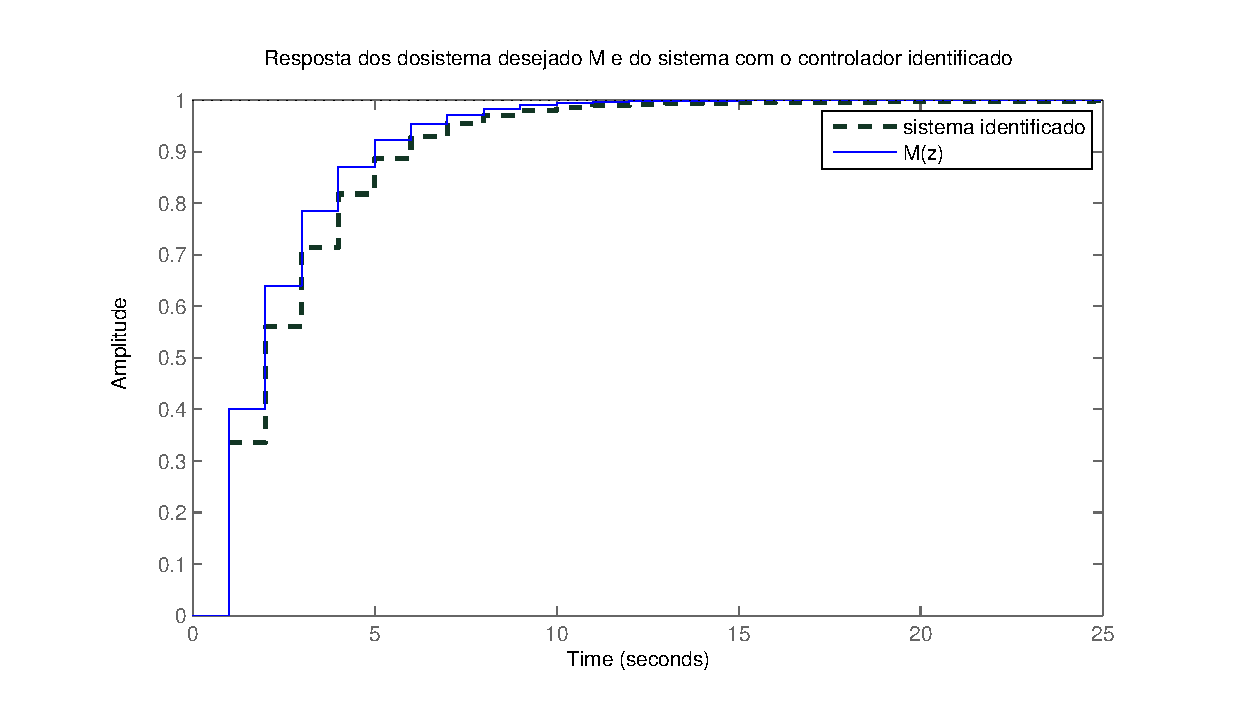
\includegraphics[width=0.95\columnwidth]{figures/vrft_nl_wiener_step.eps}
	\caption{resposta dos sistemas: desejado e obtido a um degrau unit�rio}
	\label{fig:vrft_nl_wiener_step}
\end{figure}

Na Figura (\ref{fig:vrft_nl_wiener_vw_step}) � apresentado o comportamento dos sinais de sa�da e entrada das
n�o linearidades $\Phi^{-1}(e(t))$ e $\Phi(\omega(t))$ respectivamente.

\begin{figure}[htbp] 
	\center 
	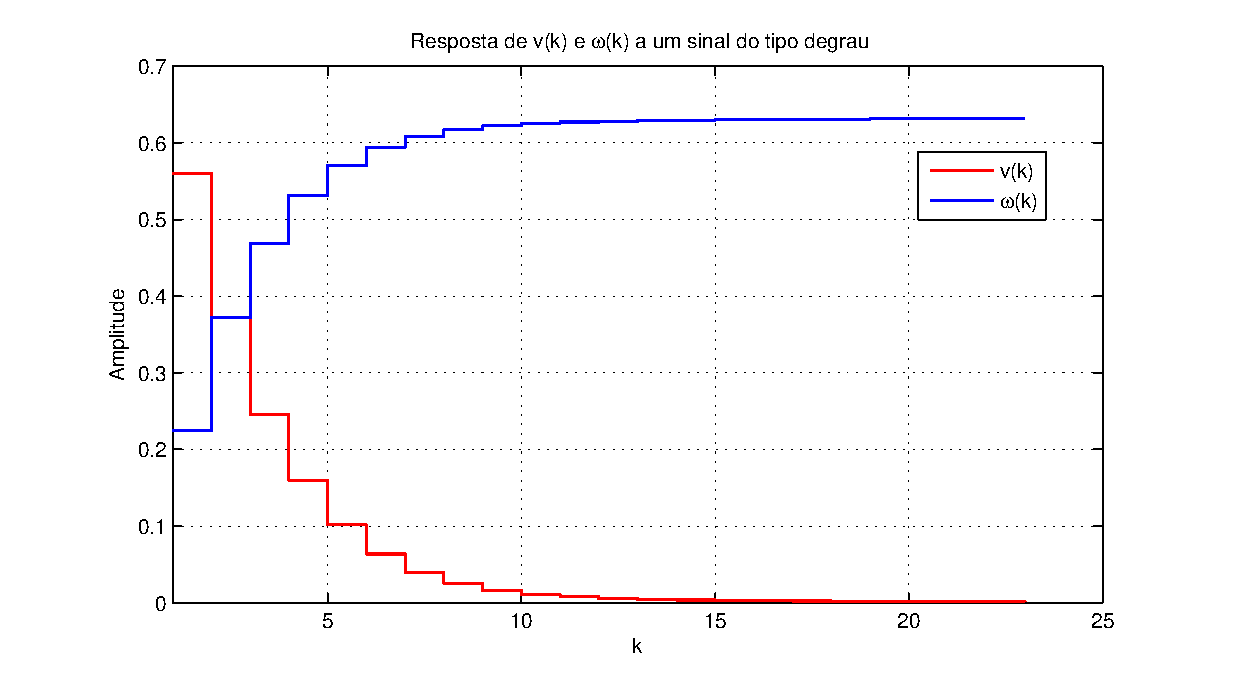
\includegraphics[width=0.95\columnwidth]{figures/vrft_nl_wiener_vw_step.eps}
	\caption{sinais $v(t)$ e $\omega(t)$ quando o sistema � alimentado por um degrau unit�rio}
	\label{fig:vrft_nl_wiener_vw_step}
\end{figure}

A rela��o entre os sinais $v(t)$ e $\omega(t)$ � apresentado na Figura (\ref{fig:vrft_nl_wiener_vw}).
Observa-se que a rela��o destes sinais � praticamente linear, garantido que a aproxima��o de $\Phi^{-1}$ foi
satisfat�ria para representar a inversa do sinal $\Phi$.

\begin{figure}[htbp] 
	\center 
	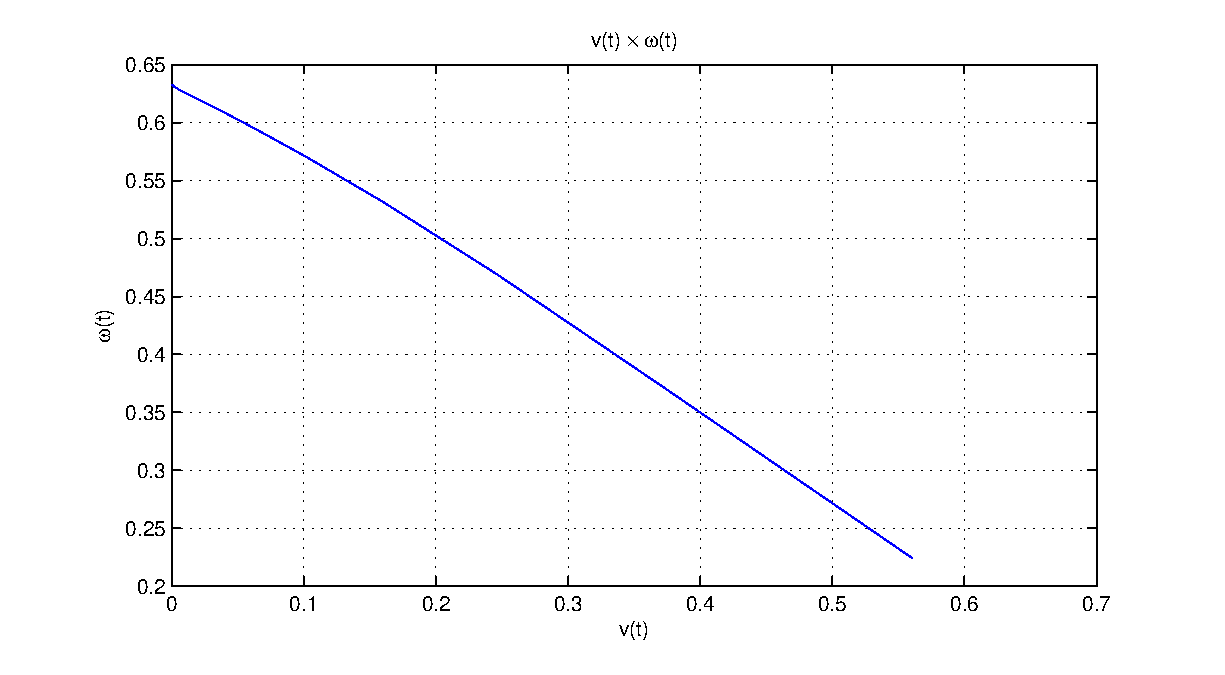
\includegraphics[width=0.95\columnwidth]{figures/vrft_nl_wiener_vw.eps}
	\caption{rela��o entre os sinais $v(t)$ e $\omega(t)$ quando o sistema � alimentado por um degrau unit�rio}
	\label{fig:vrft_nl_wiener_vw}
\end{figure}

%===============================================================================
\subsection{N�o linearidades din�micas}
\label{sec:vrft_nl_dinamic}
%===============================================================================
para um ruido de 0.005

mtheta =

    0.4000    0.5999    0.1001    0.1501    0.5000


vartheta =

   1.0e-06 *

    0.0498    0.4714    0.0581    0.4647    0.0911


stdtheta =

   1.0e-03 *

    0.2231    0.6866    0.2411    0.6817    0.3019


covtheta =

   1.0e-06 *

    0.0498    0.0585   -0.0353   -0.0362   -0.0018
    0.0585    0.4714   -0.0449   -0.3690    0.0057
   -0.0353   -0.0449    0.0581    0.0745   -0.0040
   -0.0362   -0.3690    0.0745    0.4647   -0.0070
   -0.0018    0.0057   -0.0040   -0.0070    0.0911


Jvr_nl =

   2.7291e-08


Jmr_nl =

    0.0033
ref: 

\cite{lecchini_campi_savaresi_2dof}


\cite{Guardabassi}



ruido de 0.01

mtheta =

    0.4000    0.5997    0.1000    0.1503    0.5007


vartheta =

   1.0e-04 *

    0.0609    0.6407    0.0593    0.4256    0.0970


stdtheta =

    0.0025    0.0080    0.0024    0.0065    0.0031


covtheta =

   1.0e-04 *

    0.0609    0.1062   -0.0435   -0.0642   -0.0062
    0.1062    0.6407   -0.0792   -0.4292    0.0071
   -0.0435   -0.0792    0.0593    0.0902   -0.0097
   -0.0642   -0.4292    0.0902    0.4256   -0.0194
   -0.0062    0.0071   -0.0097   -0.0194    0.0970


Jvr_nl =

   1.9177e-06


Jmr_nl =

    0.0148











































\input{tex/chapters/vrft_conclusions}
%===============================================================================

